\documentclass{ximera}

 

\usepackage{epsfig}

\graphicspath{
  {./}
  {figures/}
}

\usepackage{morewrites}
\makeatletter
\newcommand\subfile[1]{%
\renewcommand{\input}[1]{}%
\begingroup\skip@preamble\otherinput{#1}\endgroup\par\vspace{\topsep}
\let\input\otherinput}
\makeatother

\newcommand{\includeexercises}{\directlua{dofile("/home/jim/linearAlgebra/laode/exercises.lua")}}

%\newcounter{ccounter}
%\setcounter{ccounter}{1}
%\newcommand{\Chapter}[1]{\setcounter{chapter}{\arabic{ccounter}}\chapter{#1}\addtocounter{ccounter}{1}}

%\newcommand{\section}[1]{\section{#1}\setcounter{thm}{0}\setcounter{equation}{0}}

%\renewcommand{\theequation}{\arabic{chapter}.\arabic{section}.\arabic{equation}}
%\renewcommand{\thefigure}{\arabic{chapter}.\arabic{figure}}
%\renewcommand{\thetable}{\arabic{chapter}.\arabic{table}}

%\newcommand{\Sec}[2]{\section{#1}\markright{\arabic{ccounter}.\arabic{section}.#2}\setcounter{equation}{0}\setcounter{thm}{0}\setcounter{figure}{0}}

\newcommand{\Sec}[2]{\section{#1}}

\setcounter{secnumdepth}{2}
%\setcounter{secnumdepth}{1} 

%\newcounter{THM}
%\renewcommand{\theTHM}{\arabic{chapter}.\arabic{section}}

\newcommand{\trademark}{{R\!\!\!\!\!\bigcirc}}
%\newtheorem{exercise}{}

\newcommand{\dfield}{{\sf dfield9}}
\newcommand{\pplane}{{\sf pplane9}}

\newcommand{\EXER}{\section*{Exercises}}%\vspace*{0.2in}\hrule\small\setcounter{exercise}{0}}
\newcommand{\CEXER}{}%\vspace{0.08in}\begin{center}Computer Exercises\end{center}}
\newcommand{\TEXER}{} %\vspace{0.08in}\begin{center}Hand Exercises\end{center}}
\newcommand{\AEXER}{} %\vspace{0.08in}\begin{center}Hand Exercises\end{center}}

% BADBAD: \newcommand{\Bbb}{\bf}

\newcommand{\R}{\mbox{$\Bbb{R}$}}
\newcommand{\C}{\mbox{$\Bbb{C}$}}
\newcommand{\Z}{\mbox{$\Bbb{Z}$}}
\newcommand{\N}{\mbox{$\Bbb{N}$}}
\newcommand{\D}{\mbox{{\bf D}}}
\usepackage{amssymb}
%\newcommand{\qed}{\hfill\mbox{\raggedright$\square$} \vspace{1ex}}
%\newcommand{\proof}{\noindent {\bf Proof:} \hspace{0.1in}}

\newcommand{\setmin}{\;\mbox{--}\;}
\newcommand{\Matlab}{{M\small{AT\-LAB}} }
\newcommand{\Matlabp}{{M\small{AT\-LAB}}}
\newcommand{\computer}{\Matlab Instructions}
\newcommand{\half}{\mbox{$\frac{1}{2}$}}
\newcommand{\compose}{\raisebox{.15ex}{\mbox{{\scriptsize$\circ$}}}}
\newcommand{\AND}{\quad\mbox{and}\quad}
\newcommand{\vect}[2]{\left(\begin{array}{c} #1_1 \\ \vdots \\
 #1_{#2}\end{array}\right)}
\newcommand{\mattwo}[4]{\left(\begin{array}{rr} #1 & #2\\ #3
&#4\end{array}\right)}
\newcommand{\mattwoc}[4]{\left(\begin{array}{cc} #1 & #2\\ #3
&#4\end{array}\right)}
\newcommand{\vectwo}[2]{\left(\begin{array}{r} #1 \\ #2\end{array}\right)}
\newcommand{\vectwoc}[2]{\left(\begin{array}{c} #1 \\ #2\end{array}\right)}

\newcommand{\ignore}[1]{}


\newcommand{\inv}{^{-1}}
\newcommand{\CC}{{\cal C}}
\newcommand{\CCone}{\CC^1}
\newcommand{\Span}{{\rm span}}
\newcommand{\rank}{{\rm rank}}
\newcommand{\trace}{{\rm tr}}
\newcommand{\RE}{{\rm Re}}
\newcommand{\IM}{{\rm Im}}
\newcommand{\nulls}{{\rm null\;space}}

\newcommand{\dps}{\displaystyle}
\newcommand{\arraystart}{\renewcommand{\arraystretch}{1.8}}
\newcommand{\arrayfinish}{\renewcommand{\arraystretch}{1.2}}
\newcommand{\Start}[1]{\vspace{0.08in}\noindent {\bf Section~\ref{#1}}}
\newcommand{\exer}[1]{\noindent {\bf \ref{#1}}}
\newcommand{\ans}{}
\newcommand{\matthree}[9]{\left(\begin{array}{rrr} #1 & #2 & #3 \\ #4 & #5 & #6
\\ #7 & #8 & #9\end{array}\right)}
\newcommand{\cvectwo}[2]{\left(\begin{array}{c} #1 \\ #2\end{array}\right)}
\newcommand{\cmatthree}[9]{\left(\begin{array}{ccc} #1 & #2 & #3 \\ #4 & #5 &
#6 \\ #7 & #8 & #9\end{array}\right)}
\newcommand{\vecthree}[3]{\left(\begin{array}{r} #1 \\ #2 \\
#3\end{array}\right)}
\newcommand{\cvecthree}[3]{\left(\begin{array}{c} #1 \\ #2 \\
#3\end{array}\right)}
\newcommand{\cmattwo}[4]{\left(\begin{array}{cc} #1 & #2\\ #3
&#4\end{array}\right)}

\newcommand{\Matrix}[1]{\ensuremath{\left(\begin{array}{rrrrrrrrrrrrrrrrrr} #1 \end{array}\right)}}

\newcommand{\Matrixc}[1]{\ensuremath{\left(\begin{array}{cccccccccccc} #1 \end{array}\right)}}



\renewcommand{\labelenumi}{\theenumi)}
\newenvironment{enumeratea}%
{\begingroup
 \renewcommand{\theenumi}{\alph{enumi}}
 \renewcommand{\labelenumi}{(\theenumi)}
 \begin{enumerate}}
 {\end{enumerate}\endgroup}



\newcounter{help}
\renewcommand{\thehelp}{\thesection.\arabic{equation}}

%\newenvironment{equation*}%
%{\renewcommand\endequation{\eqno (\theequation)* $$}%
%   \begin{equation}}%
%   {\end{equation}\renewcommand\endequation{\eqno \@eqnnum
%$$\global\@ignoretrue}}

%\input{psfig.tex}

\author{Martin Golubitsky and Michael Dellnitz}

%\newenvironment{matlabEquation}%
%{\renewcommand\endequation{\eqno (\theequation*) $$}%
%   \begin{equation}}%
%   {\end{equation}\renewcommand\endequation{\eqno \@eqnnum
% $$\global\@ignoretrue}}

\newcommand{\soln}{\textbf{Solution:} }
\newcommand{\exercap}[1]{\centerline{Figure~\ref{#1}}}
\newcommand{\exercaptwo}[1]{\centerline{Figure~\ref{#1}a\hspace{2.1in}
Figure~\ref{#1}b}}
\newcommand{\exercapthree}[1]{\centerline{Figure~\ref{#1}a\hspace{1.2in}
Figure~\ref{#1}b\hspace{1.2in}Figure~\ref{#1}c}}
\newcommand{\para}{\hspace{0.4in}}

\renewenvironment{solution}{\suppress}{\endsuppress}

\ifxake
\newenvironment{matlabEquation}{\begin{equation}}{\end{equation}}
\else
\newenvironment{matlabEquation}%
{\let\oldtheequation\theequation\renewcommand{\theequation}{\oldtheequation*}\begin{equation}}%
  {\end{equation}\let\theequation\oldtheequation}
\fi

\makeatother


\title{*Second Order Equations}

\begin{document}
\begin{abstract}
\end{abstract}
\maketitle

  \label{S:SOE}

A second order constant coefficient
homogeneous\index{homogeneous} differential equation
is a differential equation of the form:
\begin{equation} \label{eq:soex1}
\ddot{x} + b\dot{x} + ax = 0,
\end{equation}
where $a$ and $b$ are real numbers.

\subsection*{Newton's Second Law}

{\em Newton's second law of motion\/} is a second order ordinary
\index{Newton's second law}
differential equation, and for this reason second order equations arise
naturally in mechanical systems.  Newton's second law states that
\begin{equation}  \label{e:2ndlaw}
F=ma
\end{equation}
where $F$ is force\index{force}, $m$ is mass\index{mass},
and $a$ is acceleration\index{acceleration}.

\subsubsection*{Newton's Second Law and Particle Motion on a Line}
\index{particle motion}

For a point mass moving along a line, \eqref{e:2ndlaw} is
\begin{equation} \label{E:F=ma}
F=m\frac{d^2x}{dt^2},
\end{equation}
where $x(t)$ is the position of the point mass at time $t$.
For example, suppose that a particle of mass $m$ is falling towards
the earth.  If we let $g$ be the gravitational constant and if we
ignore all forces except gravitation, then the force acting on that
particle is $F=-mg$.  In this case Newton's second law leads to the
second order ordinary differential equation
\begin{equation} \label{e:pointpart}
\frac{d^2x}{dt^2}+g=0.
\end{equation}

\subsubsection*{Newton's Second Law and the Motion of a Spring}
\index{spring} \index{spring!motion of}

As a second example, consider the spring model pictured in
Figure~\ref{F:spring2}.  Assume that the spring has zero mass and that
an object of mass $m$ is attached to the end of the spring.  Let $L$ be
the natural length of the spring, and let $x(t)$ measure the distance
that the spring is extended (or compressed).  It follows from Newton's
Law that \eqref{E:F=ma} is satisfied.  Hooke's law \index{Hooke's law}
states that the force $F$ acting on a spring is
\[
 F = -\kappa x,
\]
where $\kappa$ is a positive constant.  If the spring is damped by
sliding friction\index{sliding friction}, then
\[
F=-\kappa x - \mu \frac{dx}{dt},
\]
where $\mu$ is also a positive constant.  Suppose, in addition, that
an external force\index{external force} $F_{ext}(t)$ also acts on the
mass and that that
force is time-dependent.  Then the entire force acting on the mass is
\[
F=-\kappa x - \mu \frac{dx}{dt}+F_{ext}(t).
\]
By Newton's second law, the motion of the mass is described by
\begin{equation}  \label{e:springeq}
m\frac{d^2x}{dt^2} + \mu\frac{dx}{dt} + \kappa x = F_{ext}(t),
\end{equation}
which is again a second order ordinary differential equation.
\begin{figure}[thb]
      \centerline{%
      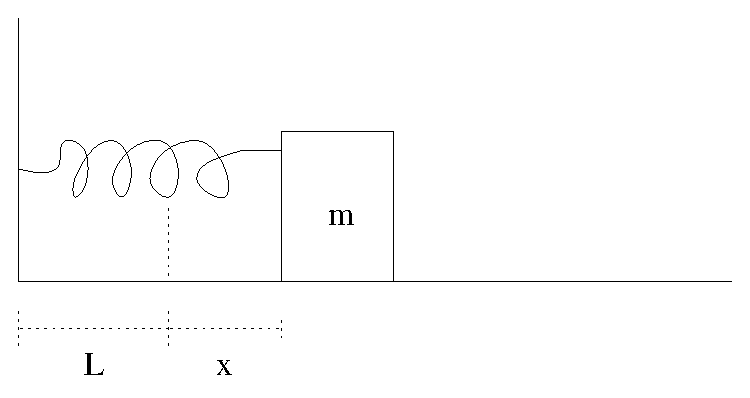
\psfig{file=../figures/spring.eps,height=1.5in}}
      \caption{Hooke's Law spring.}
      \label{F:spring2}
\end{figure}


\subsection*{A Reduction to a First Order System}
\index{first order!reduction to}

There is a simple trick that reduces a single linear second order
differential equation to a system of two linear first order equations.
For example, consider the linear homogeneous ordinary differential
equation \eqref{eq:soex1}.  To reduce this second order equation to a first order
system, just set $y=\dot{x}$.  Then \eqref{eq:soex1} becomes
\[
\dot{y} + by + ax = 0.
\]
It follows that if $x(t)$ is a solution to \eqref{eq:soex1} and
$y(t)=\dot{x}(t)$, then $(x(t),y(t))$ is a solution to
\begin{equation}  \label{e:soex1sys}
\begin{array}{rcl}
\dot{x} & = & y \\
\dot{y} & = & -ax - by.
\end{array}
\end{equation}
We can rewrite \eqref{e:soex1sys} as
\[
\dot{X} = Q X.
\]
where
\begin{equation}  \label{e:coeffmatQ}
Q =  \mattwo{0}{1}{-a}{-b}.
\end{equation}
Note that if $(x(t),y(t))$ is a solution to \eqref{e:soex1sys}, then
$x(t)$ is a solution to \eqref{eq:soex1}.  Thus solving the single
second order linear equation is exactly the same as solving the
corresponding first order linear system.

\subsubsection*{The Initial Value Problem}
\index{initial value problem!for second order equations}

To solve the homogeneous system \eqref{e:soex1sys} we need to specify
two initial conditions $X(0)=(x(0),y(0))^t$.  It follows that to
solve the single second order equation we need to specify two initial
conditions $x(0)$ and $\dot{x}(0)$; that is, we need to specify
both initial position\index{initial position} and
initial velocity\index{initial velocity}.

\subsection*{The General Solution}

There are two ways in which we can solve
the second order homogeneous equation \eqref{eq:soex1}.  First,
we know how to solve the system \eqref{e:soex1sys} by finding the
eigenvalues and eigenvectors of the coefficient matrix $Q$ in
\eqref{e:coeffmatQ}.  Second, we know from the general theory of
planar systems that solutions will have the form $x(t)=e^{\lambda_0t}$
for some scalar $\lambda_0$.  We need only determine the values of
$\lambda_0$ for which we get solutions to \eqref{eq:soex1}.

We now discuss the second approach.  Suppose that $x(t)=e^{\lambda_0t}$
is a solution to \eqref{eq:soex1}.  Substituting this form of $x(t)$ in
\eqref{eq:soex1} yields the equation
\[
\left(\lambda_0^2 + b\lambda_0 + a\right)e^{\lambda_0t} = 0.
\]
So $x(t)=e^{\lambda_0t}$ is a solution to \eqref{eq:soex1} precisely
when $p_Q(\lambda_0)=0$, where
\begin{equation} \label{E:charQ}
p_Q(\lambda) = \lambda^2 + b\lambda + a
\end{equation}
is the characteristic polynomial of the matrix $Q$ in \eqref{e:coeffmatQ}.

Suppose that $\lambda_1$ and $\lambda_2$ are distinct real roots of $p_Q$.
Then the general solution\index{general solution} to \eqref{eq:soex1} is
\[
x(t) = \alpha_1e^{\lambda_1t} +  \alpha_2e^{\lambda_2t},
\]
where $\alpha_j\in\R$.

\subsubsection*{An Example with Distinct Real Eigenvalues}

For example, solve the initial value problem
\begin{equation} \label{e:ex12}
\ddot{x} + 3\dot{x} + 2x = 0
\end{equation}
with initial conditions $x(0)=0$ and $\dot{x}(0)=-2$.  The characteristic
polynomial is
\[
p_Q(\lambda) = \lambda^2 + 3\lambda + 2 = (\lambda+2)(\lambda+1),
\]
whose roots are $\lambda_1=-1$ and $\lambda_2=-2$.  So the general solution
to \eqref{e:ex12} is
\[
x(t) = \alpha_1e^{-t} + \alpha_2e^{-2t}
\]
To find the precise solution we need to solve
\[
\begin{array}{rclcl}
x(0) & = & \alpha_1 + \alpha_2 & = & 0 \\
\dot{x}(0) & = & -\alpha_1 - 2\alpha_2 & = & -2
\end{array}
\]
So $\alpha_1 = -2$, $\alpha_2=2$, and the solution to the initial value problem
for \eqref{e:ex12} is
\[
x(t) = -2e^{-t} + 2e^{-2t}
\]

\subsubsection*{An Example with Complex Conjugate Eigenvalues}

Consider the differential equation
\begin{equation} \label{E:ex13}
\ddot{x} -2\dot{x} + 5x = 0.
\end{equation}
The roots of the characteristic polynomial associated to \eqref{E:ex13} are
$\lambda_1=1+2i$ and $\lambda_2=1-2i$.  It follows from the discussion in
the previous section that the general solution to \eqref{E:ex13} is
\[
x(t) = \RE\left(\alpha_1 e^{\lambda_1 t} + \alpha_2 e^{\lambda_2t}\right)
\]
where $\alpha_1$ and $\alpha_2$ are complex scalars.  Indeed, we can rewrite
this solution in real form (using Euler's formula) as
\[
x(t) = e^t\left(\beta_1\cos(2t) + \beta_2\sin(2t)\right),
\]
for real scalars $\beta_1$ and $\beta_2$.

In general, if the roots of the characteristic polynomial are
$\sigma\pm i\tau$, then the general solution to the differential equation is:
\[
x(t) = e^{\sigma t}\left(\beta_1\cos(\tau t) + \beta_2\sin(\tau t)\right).
\]

\subsubsection*{An Example with Multiple Eigenvalues}

Note that the coefficient matrix $Q$ of the associated first order system
in \eqref{e:coeffmatQ} is never a multiple of $I_2$.  It follows from the
previous section
that when the roots of the characteristic polynomial are real and equal,
the general solution has the form
\[
x(t) = \alpha_1 e^{\lambda_1t} + \alpha_2te^{\lambda_2t}.
\]

\subsubsection*{Summary}

It follows from this discussion that solutions to second order
homogeneous linear equations are either a linear combination of two
exponentials (real unequal eigenvalues), $\alpha+\beta t$ times one
exponential (real equal eigenvalues), or a time periodic function times
an exponential (complex eigenvalues).

In particular, if the real part
of the complex eigenvalues is zero, then the solution is time periodic.
The frequency of this periodic solution is often called the {\em internal
frequency}\index{frequency!internal}, a point
that is made more clearly in the next example.


\subsection*{Solving the Spring Equation}

Consider the equation for the frictionless spring without
external forcing.  From \eqref{e:springeq} we get  \index{spring equation}
\index{spring!undamped}
\begin{equation} \label{ex:uspring}
m\ddot{x} + \kappa x = 0.
\end{equation}
where $\kappa>0$.  The roots are $\lambda_1=\sqrt{\frac{\kappa}{m}}i$
and $\lambda_2=-\sqrt{\frac{\kappa}{m}}i$.  So the general solution is
\[
x(t) = \alpha\cos(\tau t) + \beta\sin(\tau t),
\]
where $\tau=\sqrt{\frac{\kappa}{m}}$.  Under these assumptions the
motion of the spring is time periodic with period $\frac{2\pi}{\tau}$
or internal frequency $\frac{\tau}{2\pi}$.  In particular, the solution
satisfying initial conditions $x(0)=1$ and $\dot{x}(0)=0$ (the spring is
extended one unit in distance and released with no initial velocity) is
\[
x(t) = \cos(\tau t).
\]
The graph of this function when $\tau=1$ is given on the
left in Figure~\ref{F:springp}.
\begin{figure*}[htb]
           \centerline{%
           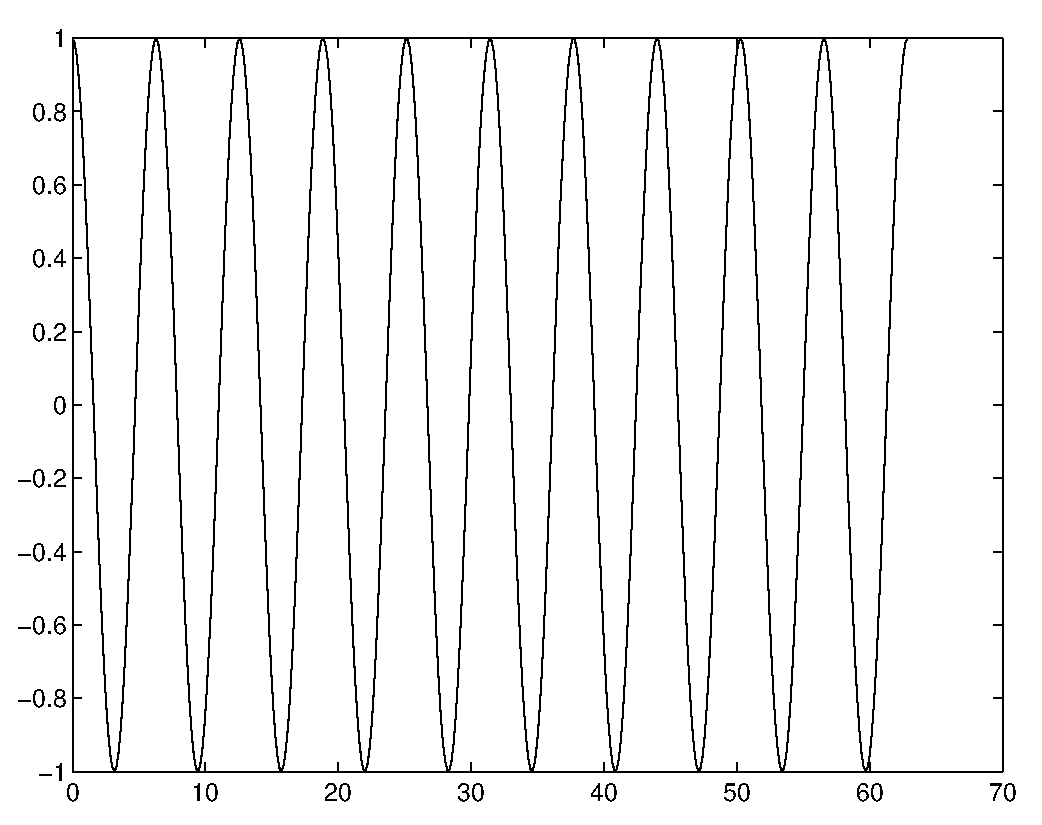
\psfig{file=../figures/springp.eps,width=3.0in}
           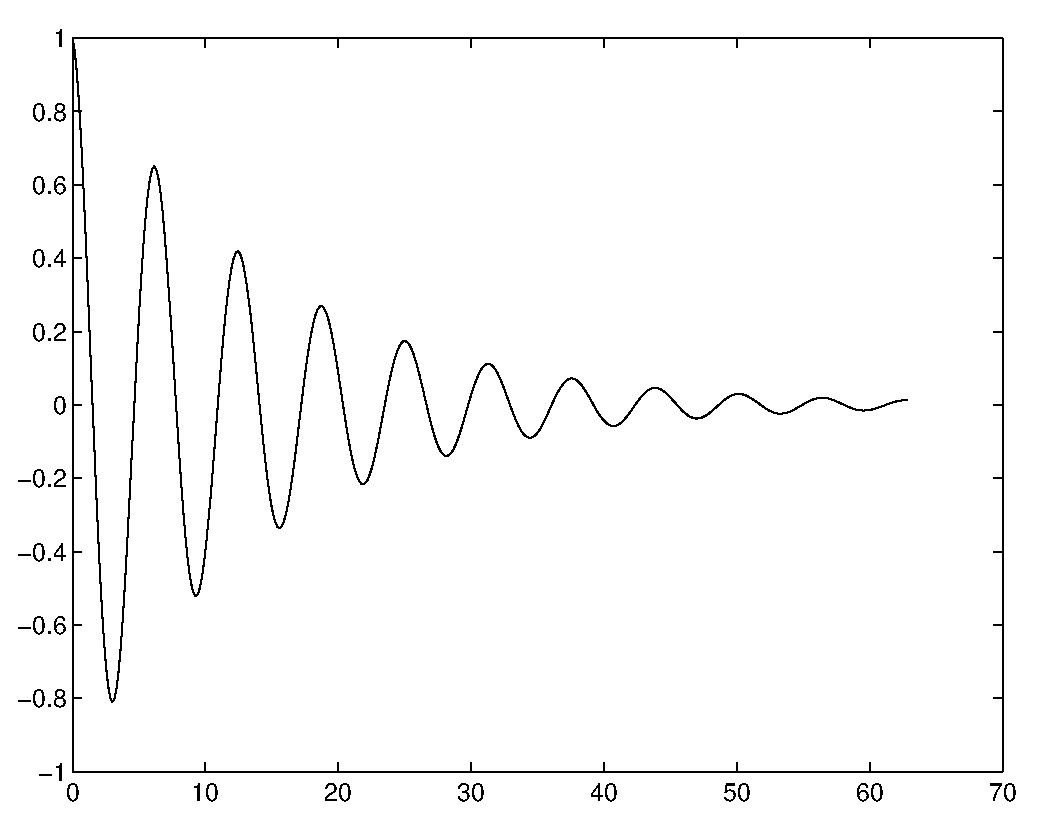
\psfig{file=../figures/springpd.eps,width=3.0in}}
           \caption{(Left) Graph of solution to undamped spring
	equation with initial conditions $x(0)=1$ and $\dot{x}(0)=0$.
	(Right) Graph of solution to damped spring equation with the
	same initial conditions.}
           \label{F:springp}
\end{figure*}

If a small amount of friction is added, then the spring equation is
\index{spring!damped}
\[
m\ddot{x} + \mu \dot{x} +\kappa x = 0
\]
where $\mu>0$ is small.  Since the eigenvalues of the characteristic
polynomial are $\lambda=\sigma\pm i\tau$ where
\[
\sigma = -\frac{\mu}{2m} < 0 \AND \tau =\sqrt{\frac{\kappa}{m}
-\left(\frac{\mu}{2m}\right)^2},
\]
the general solution is
\[
x(t) = e^{\sigma t}(\alpha\cos(\tau t) + \beta\sin(\tau t)).
\]
Since $\sigma<0$, these solutions oscillate but damp down to zero.  In
particular, the solution satisfying initial conditions $x(0)=1$ and
$\dot{x}(0)=0$ is
\[
x(t) = e^{-\mu t/2m}
\left(\cos(\tau t)-\frac{\mu}{2m\tau}\sin(\tau t)\right).
\]
The graph of this solution when $\tau=1$ and $\frac{\mu}{2m}=0.07$ is
given in Figure~\ref{F:springp} (right).  Compare the solutions for the
undamped and damped springs.

\EXER

\TEXER

\begin{exercise} \label{c6.7.1}
By direct integration solve the differential equation \eqref{e:pointpart}
for a point particle moving only under the influence of gravity.  Find the
solution for a particle starting at a height of $10$ feet above ground with
an upward velocity of $20$ feet/sec.  At what time will the particle hit
the ground?  (Recall that acceleration due to gravity is $32$ feet/sec$^2$.)
\end{exercise}

\begin{exercise} \label{c6.7.2}
By direct integration solve the differential equation \eqref{e:pointpart}
for a point particle moving only under the influence of gravity.  Show
that the solution is
\[
x(t) = -\frac{1}{2}gt^2 + v_0t + x_0
\]
where $x_0$ is the initial position of the particle and $v_0$ is the initial
velocity.
\end{exercise}

\noindent  In Exercises~\ref{c6.6.hoa} -- \ref{c6.6.hoc} find the general
solution to the given differential equation.
\begin{exercise} \label{c6.6.hoa}
$\ddot{x} + 2\dot{x} - 3x = 0$.
\end{exercise}
\begin{exercise} \label{c6.6.hob}
$\ddot{x} - 6\dot{x} + 9x = 0$.
In addition, find the solution to this equation satisfying
initial values $x(1)=1$ and $\dot{x}(1)=0$.
\end{exercise}
\begin{exercise} \label{c6.6.hoc}
$\ddot{x} + 2\dot{x} + 2x = 0$.
\end{exercise}

\begin{exercise} \label{c6.7.3}
Prove that a nonzero solution to a second order linear differential equation
with constant coefficients cannot be identically equal to zero on a nonempty
interval.
\end{exercise}

\begin{exercise} \label{c6.7.4}
Let $r>0$ and $w>0$ be constants, and let $x(t)$ be a solution to the
differential equation
\[
\ddot{x} + r\dot{x} + wx = 0.
\]
Show that $\dps\lim_{t\to\infty} x(t) = 0$.
\end{exercise}

\noindent In Exercises~\ref{c6.6.tfa} -- \ref{c6.6.tfc}, let $x(t)$ be a
solution to the second order linear homogeneous differential equation
\eqref{eq:soex1}.  Determine whether the given statement is {\em true\/}
or {\em false}.
\begin{exercise} \label{c6.6.tfa}
If $x(t)$ is nonconstant and time periodic, then the
roots of the characteristic polynomial are purely imaginary.
\end{exercise}
\begin{exercise} \label{c6.6.tfb}
If $x(t)$ is constant in $t$, then one of the roots of
the characteristic polynomial is zero.
\end{exercise}
\begin{exercise} \label{c6.6.tfc}
If $x(t)$ is not bounded, then the roots of the characteristic
polynomial are equal.
\end{exercise}

\begin{exercise} \label{c3.5.5}
Consider the second order differential equation
\begin{equation}  \label{E:2ndorder}
\frac{d^2x}{dt^2} + a(x)\frac{dx}{dt} + b(x) = 0.
\end{equation}
Let $y(t)=\dot{x}(t)$ and show that \eqref{E:2ndorder} may be
rewritten as a first order coupled system in $x(t)$ and $y(t)$
as follows:
\begin{eqnarray*}
\dot{x} & = & y \\
\dot{y} & = & -b(x) - a(x) y.
\end{eqnarray*}
\end{exercise}


\CEXER

\begin{exercise} \label{c6.7.5}
Use {\sf pplane8} to compute solutions to the system corresponding to the
spring equations with small sliding friction.  Plot the time series (in $x$)
of the solution and observe the oscillating and damping of the solution.
\end{exercise}







\end{document}
